%part2.tex
\part{\LaTeX{}图形宏集}\label{part:graphicbundle}

这一部分简要介绍了 \LaTeX{} 图形宏集。
更多细节可以参考图形宏集文档 \cite{grfguide} 或者 \emph{\LaTeX{} Graphics Companion}\cite{Goossens1997}。

\section{图像文件加载}\label{sec:graphicsinclusion}

导入图像需要使用 \pkg{graphicx} 宏包的 \cmd{includegraphics} 命令,语法为
\begin{lstlisting}[frame=shadowbox]
\includegraphics[选项]{文件}
\end{lstlisting}
这里\emph{选项} 在表~\ref{tab:opt}、\ref{tab:cropopt}、\ref{tab:boolopt} 中列出。
因为 \cmd{includegraphics} 不会结束当前段落,所以它能够在文本中放置图形如
 
\includegraphics[width=12pt]{recycle} 和 
\includegraphics[width=12pt]{illusion}。

\subsection{图形驱动}\label{ssec:driver}
用户必须指定一个图形驱动以告诉图形宏包如何处理导入的图像。
目前\LaTeX{} 图形宏集支持18种不同的驱动
\footnote{
	到目前(2016年)为止,支持的驱动数已经超过了20种。——译注
	},
不过,本文档只涉及两种最常用的驱动:
\prgname{dvips} 类型文档所用的 \prgname{dvips} 驱动
\footnote{使用 \prgname{latex} 命令将 \LaTeX{} 文件处理成 \file{dvi} 文件后,
	\prgname{dvips} 随后就将其转成 PostScript 格式。},
以及 \pdfLaTeX{} 文档所用的 \prgname{pdftex} 驱动。
如果用户使用的是这两种驱动之一,一般不用显示地指明,
因为绝大部分 \LaTeX{} 发行版中的 \file{graphics.cfg} 可以自动识别正确的驱动
\footnote{\file{graphics.cfg} 文件会检测文件是由 \prgname{latex} 还是 \prgname{pdflatex} 编译,
	对于 \prgname{latex} 会指定 \opt{dvips} 选项,
	对于 \prgname{pdflatex} 会指定 \opt{pdftex} 选项。}。

如果用户想要指定一个驱动,可以用以下三种方式
\marginpar{指定驱动}
\begin{enumerate}
	\item 默认值在 \file{graphics.cfg} 文件中指定。
	\item 任何通过 \cmd{documentclass} 的选项指定的驱动会覆盖由 \file{graphics.cfg} 文件指定的驱动。
	\item 任何由 \cmdM{usepackage}{graphics} 的选项指定的驱动会覆盖前两种方式指定的驱动。
\end{enumerate}

\subsection{DVIPS 模式下图像加载}
\prgname{dvips} 模式下支持最好的图像格式是 \file{eps}。
当使用 \prgname{latex} 编译文件时,下面的命令
\begin{lstlisting}
\includegraphics{file.eps}
\end{lstlisting}
会从 \file{file.eps} 文件中按照自然大小导入图像。
如果文件名没有扩展名,
\begin{lstlisting}
\includegraphics{file}
\end{lstlisting}
那么 \cmd{includegraphics} 会按照 \cmd{DeclareGraphicsExtensions} 扩展名列表中自动加上扩展名
(见~\pageref{ssec:deextension} 的第~\ref{ssec:deextension} 节)。

\subsection[pdfLaTeX 模式下的图像加载]{\pdfLaTeX{} 模式下的图像加载}
\pdfTeX{} 支持直接导入 \file{pdf}、\file{png}、\file{jpeg} 和 MetaPost 图像。
当使用 \prgname{pdflatex} 编译时,下面的命令
\begin{lstlisting}
\includegraphics{file.pdf}
\includegraphics{file.png}
\includegraphics{file.jpg}
\includegraphics{file.mps}
\end{lstlisting}
会按照自然尺寸大小导入 \file{pdf} 文件 \file{file.pdf}、
\file{png} 文件 \file{file.png}、
\file{jpeg} 文件 \file{file.jpg}
以及 MetaPost 文件 \file{file.mps}。
如果文件名没有扩展名
\begin{lstlisting}
\includegraphics{file.eps}
\end{lstlisting}
那么 \cmd{includegraphics} 会按照 \cmd{DeclareGraphicsExtensions} 扩展名列表中自动加上扩展名
(见~\pageref{ssec:deextension} 的第~\ref{ssec:deextension} 节)。

\subsection{同时供 \LaTeX{} 和 \pdfLaTeX{} 编译的文档 }\label{ssec:latexandpdflatex}
很多情况下要求文档同时可以由 \LaTeX{} 或 \pdfLaTeX{} 编译。
要求 PostScript 输出时使用 \LaTeX{} 编译和 \prgname{dvips} 驱动,
要求 \file{pdf} 输出时则使用 \pdfLaTeX{} 编译。
在这两种方式之间切换会改变两件事情。
\begin{itemize}
	\item 合适的 \pkg{graphicx} 驱动会改变。
	\item 可以直接导入的图像类型会改变。
\end{itemize}
使用如下步骤会调整这些,这样一份文档可以同时由 \LaTeX{} 和 \pdfLaTeX{} 编译。
\begin{enumerate}
	\item 对于每一份要导入的图像都创建两个副本\footnote{
		有时使用 \prgname{PurifyEPS} (见 \pageref{ssec:purifyeps} 页的第~\ref{ssec:purifyeps} 节) 可以创建一个文件并可以同时供 \LaTeX{} 和 \pdfLaTeX{} 使用。}:
	\begin{enumerate}
		\item 一份 \file{eps} 版本,当使用 \prgname{latex} 编译时会导入。
		\item 一份 \file{png}、\file{pdf}、\file{jpeg} 或者 MetaPost 版本,
		当使用 \prgname{pdflatex} 编译时会导入。
	\end{enumerate}
	
	\item 不要在 \cmd{documentclass} 或者 \cmdM{usepackage}{graphicx} 命令中指定 \opt{dvips} 或者 \opt{pdftex} 选项。
	\file{graphic.cfg} 文件会自动传递合适的选项给 \pkg{graphicx} 宏包。
	
	\item 当使用 \cmd{includegraphics} 命令插图时,
	不要指定扩展名。例如
\begin{lstlisting}
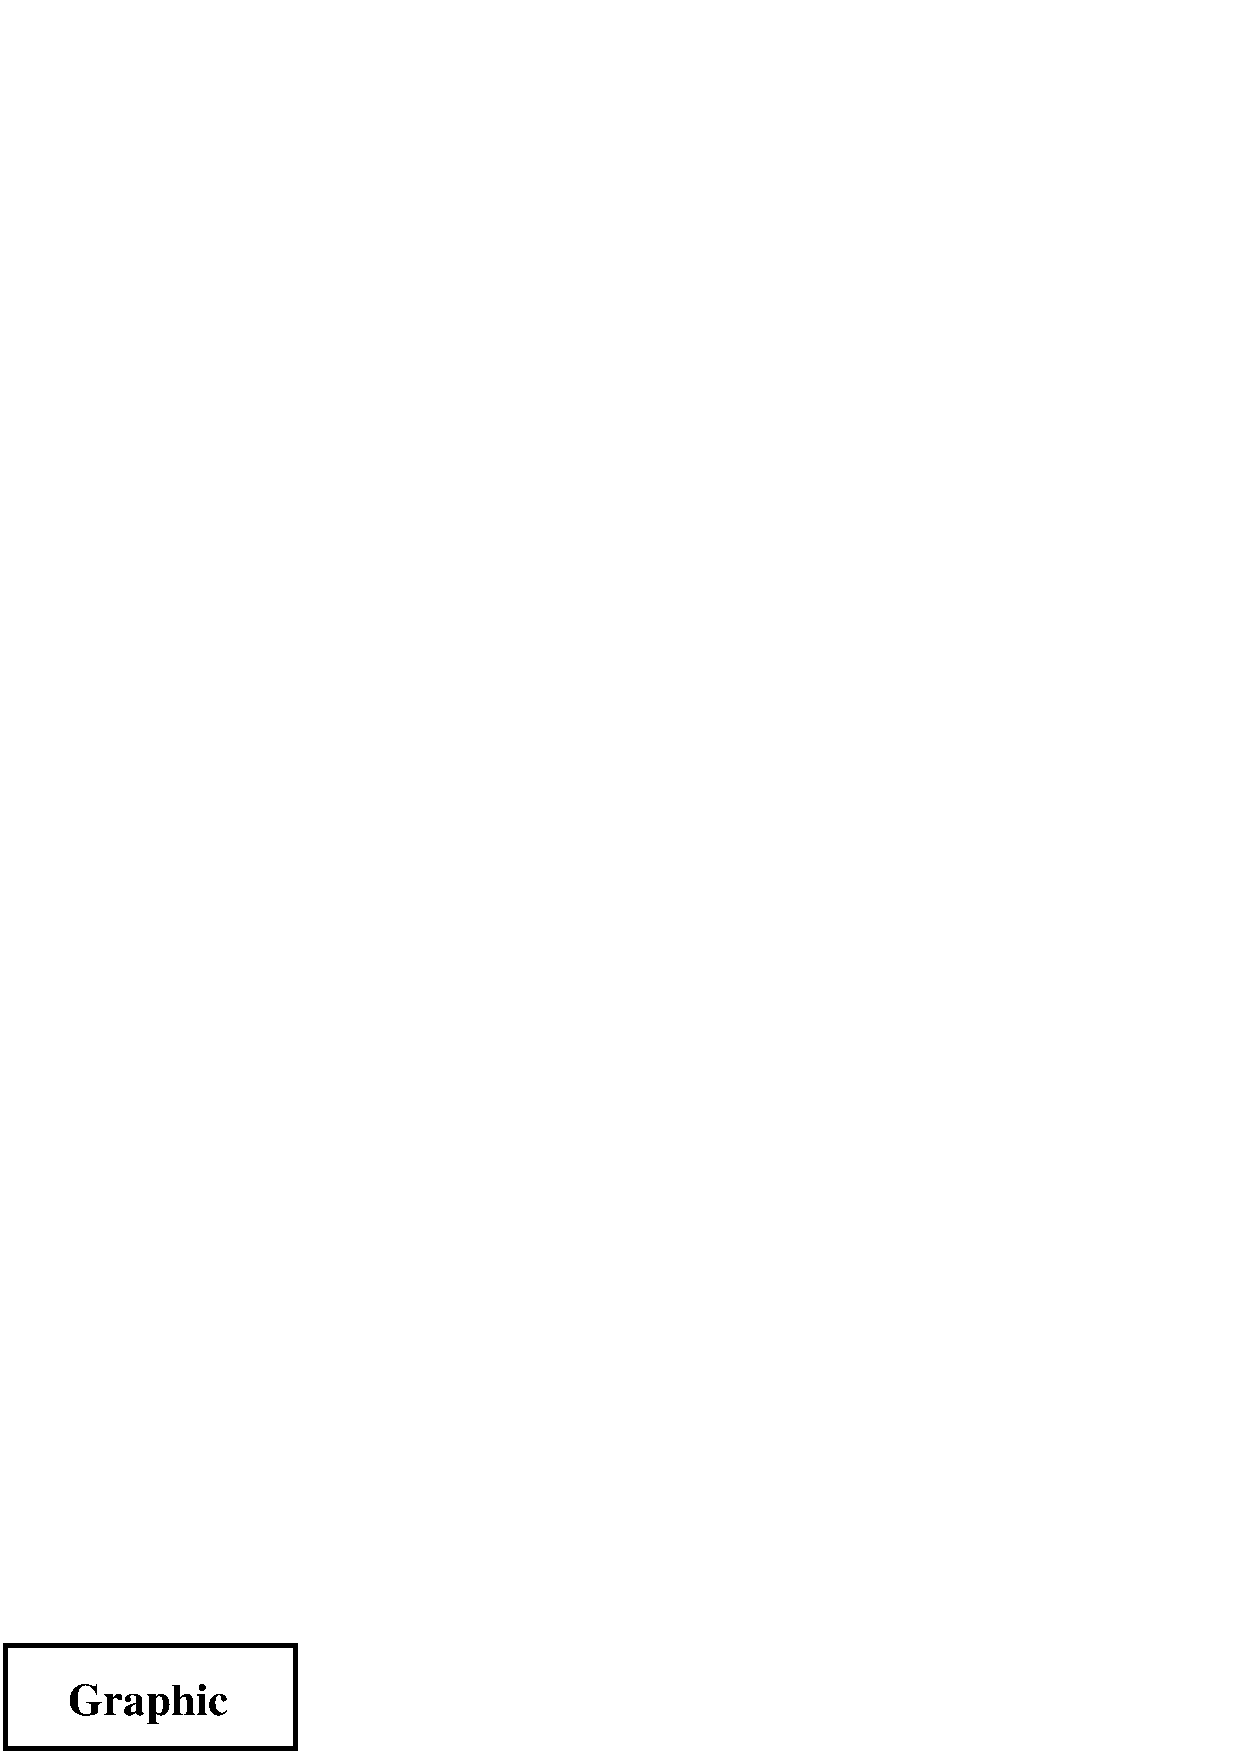
\includegraphics{graphic}
\end{lstlisting}
	定义在 \file{dvips.def} 中的默认扩展名列表会使得 \LaTeX{} 导入图像 \file{eps} 版本,
	而定义在 \file{pdftex.def} 中的默认扩展名列表会使得 \pdfLaTeX{} 导入图像的 \file{png}、\file{pdf}、\file{jpeg} 或者 MetaPost 版本
	(见~\pageref{ssec:deextension} 的第~\ref{ssec:deextension} 节)。
	
	\item 不要直接使用 \pkg{psfrag}。如果需要进行 \pkg{psfrag} 替换,
	使用~\pageref{sssec:psfrag-pdftex} 页的第~\ref{sssec:psfrag-pdftex} 节介绍的方法。
\end{enumerate}

\subsubsection{使用 \pkg{ifpdf} 宏包的条件代码}
\pkgi{ifpdf} 宏包的 \cmdi{ifpdf} 命令会检测文档是否由 \prgname{pdflatex} 编译
\footnote{
	历史上,有一种检测方法是基于 \cmd{pdfoutput} 仅在使用 \pdfLaTeX{} 时才有定义这一事实。
	然而,现在绝大部分 \TeX{} 发行版中的 \prgname{latex} 命令实际上是在 \file{dvi} 模式下执行 \pdfLaTeX{}。
	此时无论用\prgname{latex} 和 \prgname{pdflatex} 中的哪种来编译,\cmd{pdfoutput} 都有定义。
	\pkg{ifpdf} 宏包则提供了一个鲁棒的条件命令,可以判断文档是否直接处理成 \file{pdf} 文件,
	从而解决了这一问题。},
进而可以在文档中使用条件语句。

例如,为了精简扩展名列表(见第~\ref{ssec:deextension} 节),
可以用 \cmd{ifpdf} 命令来定制
\begin{lstlisting}
\usepackage{ifpdf}
...
\ifpdf
\DeclareGraphicsExtensions{.pdf,.png,.jpg,.mps}
\else
\DeclareGraphicsExtensions{.eps}
\fi
\end{lstlisting}

如果用户想要基于条件代码来使用不同的 \cmd{documentclass} 选项,
使用如下代码可以在 \cmd{documentclass} 之前定义 \cmd{ifpdf}
\begin{lstlisting}
\RequirePackage{ifpdf}
\ifpdf
\documentclass[pdftex]{article}
\else
\documentclass[dvips]{article}
\fi
\end{lstlisting}
这段代码当使用 \prgname{pdflatex} 时会传递 \opt{pdftex} 选项,
而使用 \prgname{latex} 编译时会传递 \opt{dvips} 选项。
不过,正如~\pageref{ssec:driver} 页的第~\ref{ssec:driver} 节所述,
这段代码实际上没有必要,因为绝大部分的发行版本会根据 \file{graphics.cfg} 文件自动处理驱动选项。


\subsection{指定宽度、高度和角度}\label{ssec:spec-width-height-angle}
如下命令
\marginpar{指定宽度}
\begin{lstlisting}
\includegraphics[width=3in]{file}
\end{lstlisting}
导入指定的图片文件,且宽度为 3英寸
\footnote{同时高度也会按相应的比例缩放——译注}。
不过,为了使图像的页面布局更具通用性,
图片宽度最好指定为可伸缩的相对长度而不是用像3英寸这样的固定尺寸
\footnote{
	预先定义的相对长度包括:\\
	\cmd{textwidth} 是文档中正文的宽度;\\
	\cmd{linewidth} 是当前环境中一行的宽度;\\
	\texttt{em} 是当前字体大写字母M的宽度;\\
	\texttt{ex} 是当前字体小写字母x的高度。}。
例如,
\begin{itemize}
	\item 如下命令将插入的图片伸缩至和当前一行文本的宽度相同:
\begin{lstlisting}
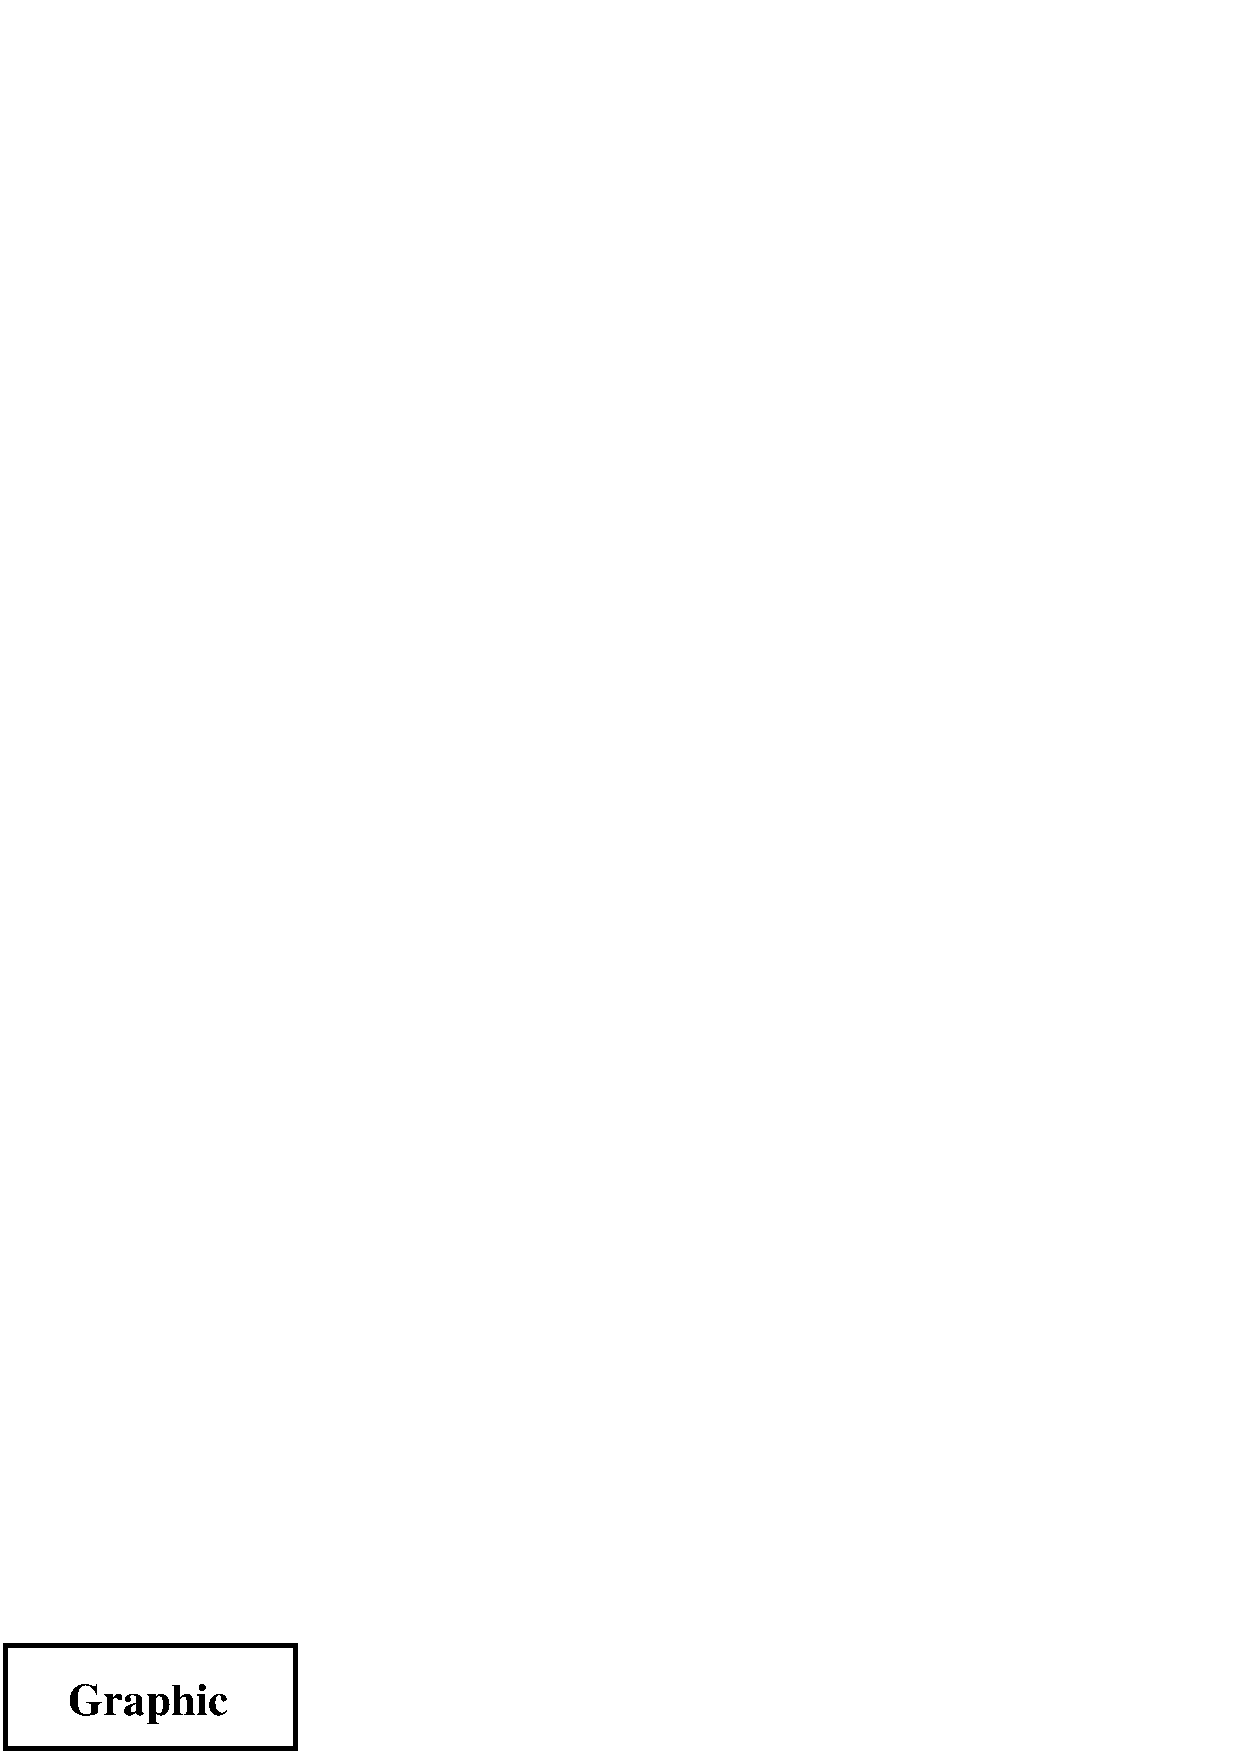
\includegraphics[width=\linewidth]{graphic}
\end{lstlisting}
	\item 如下命令使得插入图片的宽度为当前一行文本的 $80\percent$:
\begin{lstlisting}
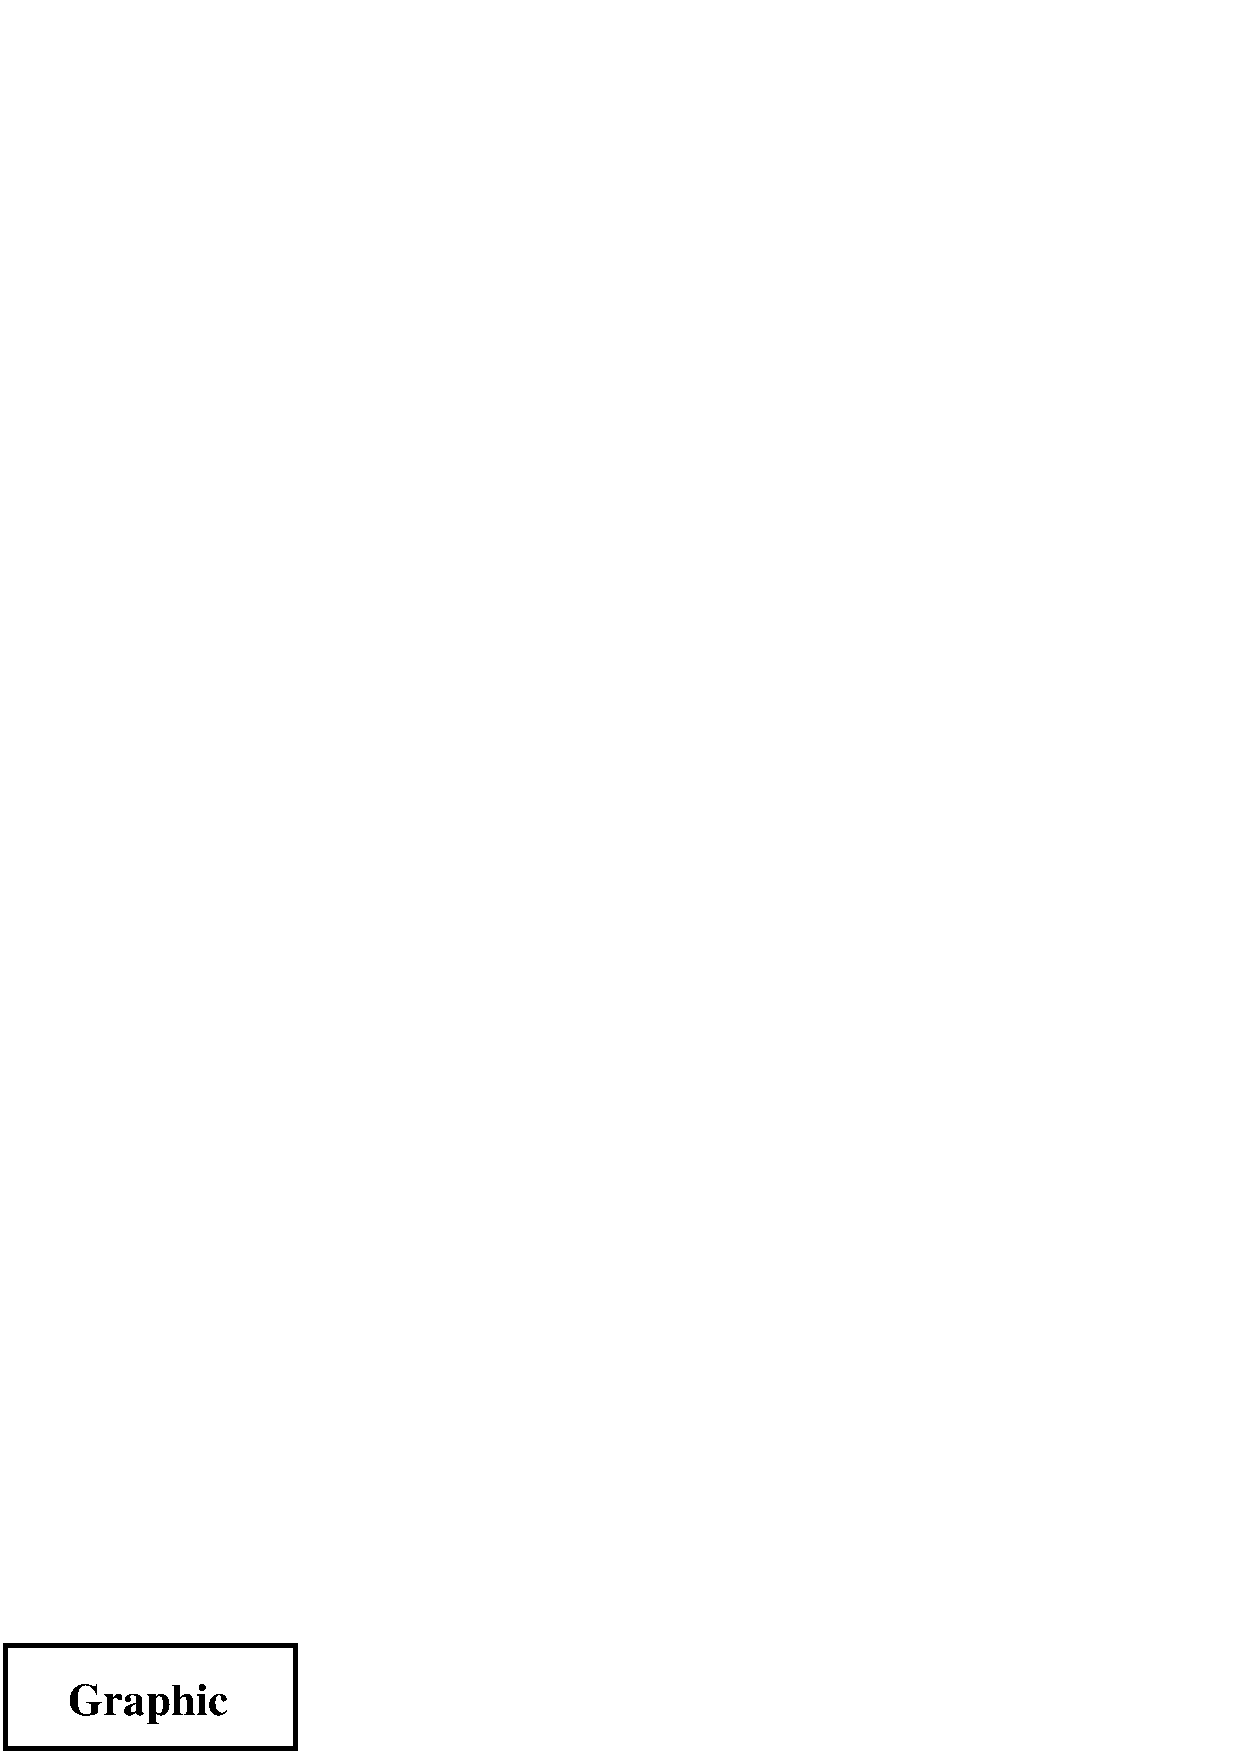
\includegraphics[width=0.80\linewidth]{graphic}
\end{lstlisting}
	\item 当与 \pkg{calc} 宏包配合使用时,
	如下命令可以使得插入图片的宽度比当前一行文本的宽度窄2英寸:
\begin{lstlisting}
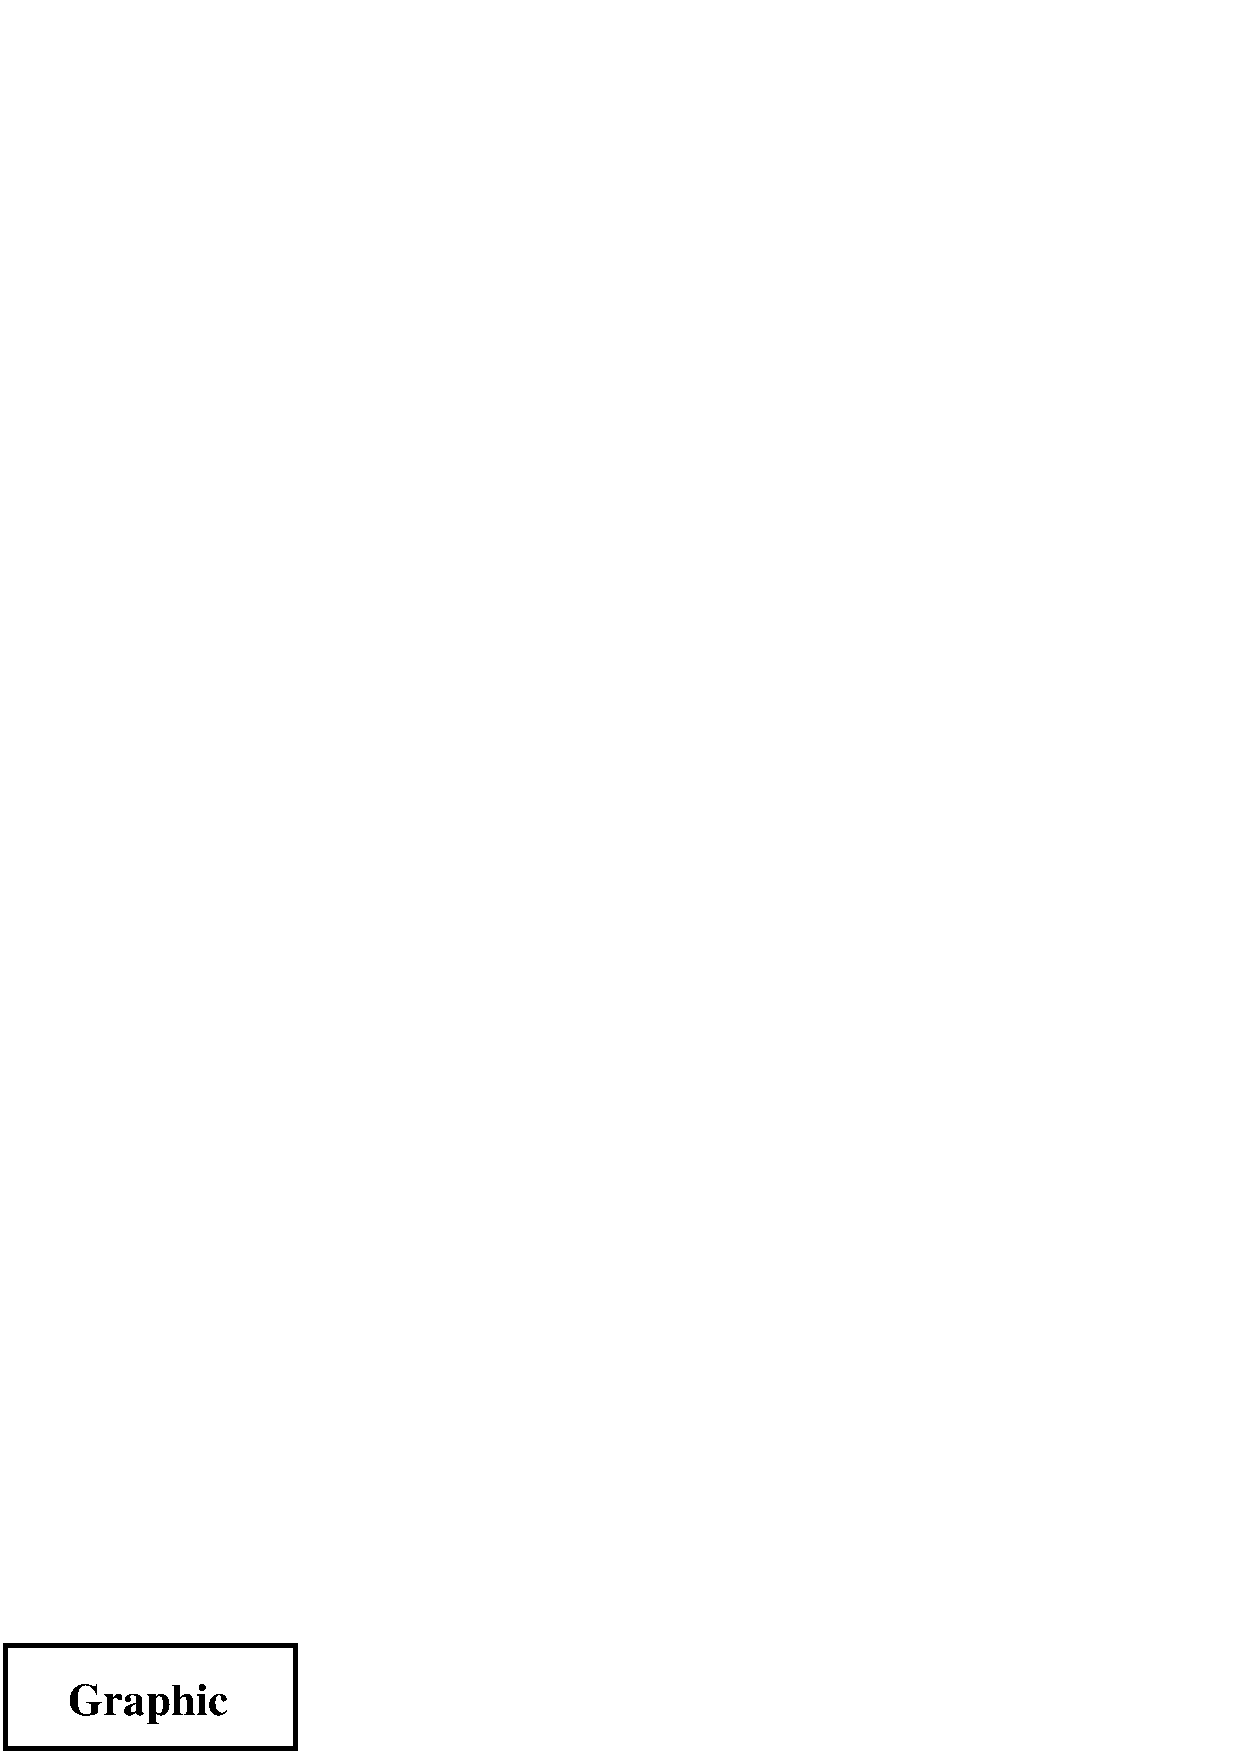
\includegraphics[width=\linewidth-2.0in]{graphic}
\end{lstlisting}
	
\end{itemize}

类似地,如下命令
\marginpar{指定高度}
\begin{lstlisting}
\includegraphics[height=2cm]{file}
\end{lstlisting}
导入指定的图片文件,且高度为2厘米。
此外,\cmd{includegraphics} 命令还有一个 \opt{totalheight} 选项来指定整体高度
(关于高度和整体高度的定义可参见第~\pageref{sec:terminology} 页的第~\ref{sec:terminology} 节)。

\cmd{includegraphics} 命令的 \opt{angle} 选项可以指定插入图像的角度:
\marginpar{指定角度}
\begin{lstlisting}
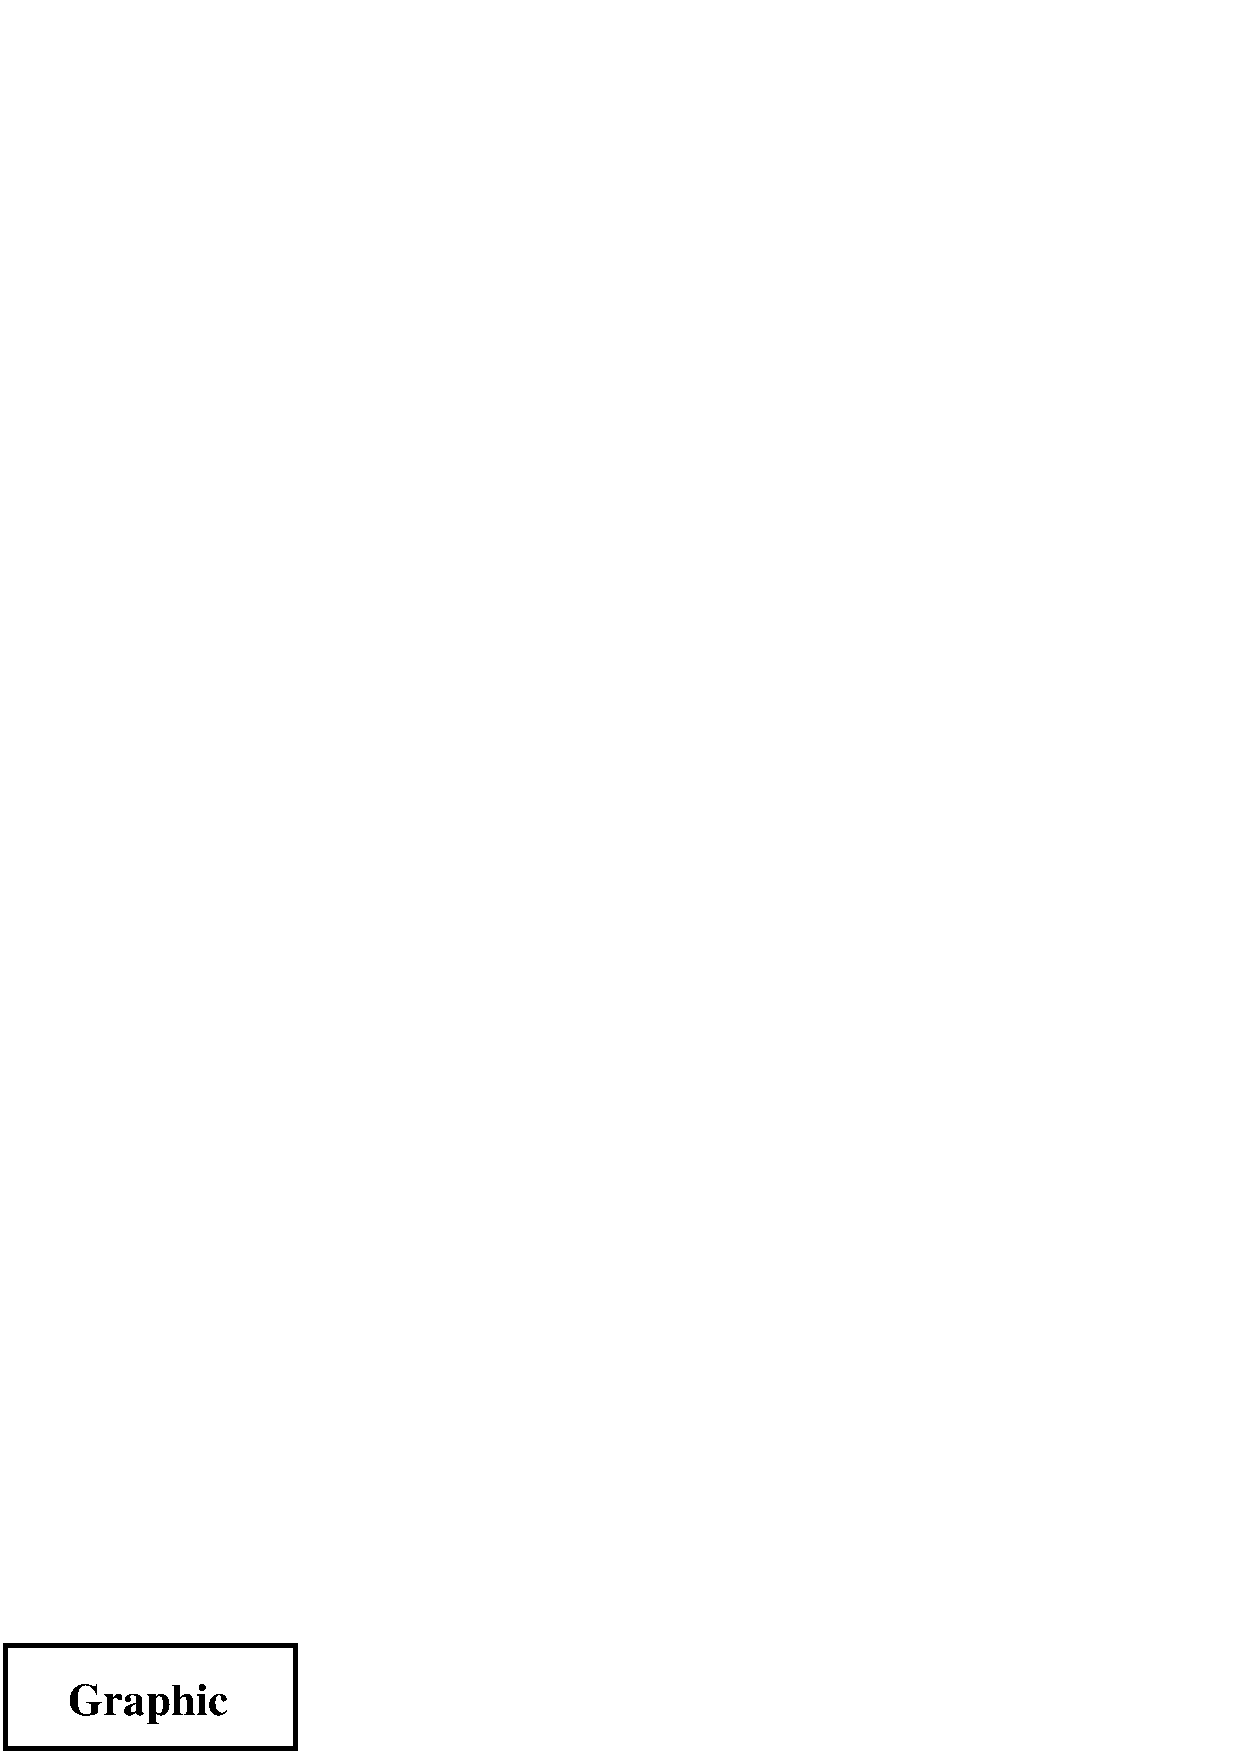
\includegraphics[angle=45]{graphic}
\end{lstlisting}
该命令会按照原始尺寸插入图片,并且按逆时针旋转45度。

\subsubsection{同时指定角度和高度/宽度}
由于 \cmd{includegraphics} 的选项是从左到右依次解释的,
所以其中指定角度和大小顺序会导致不同的效果。例如
\begin{lstlisting}
\begin{center}
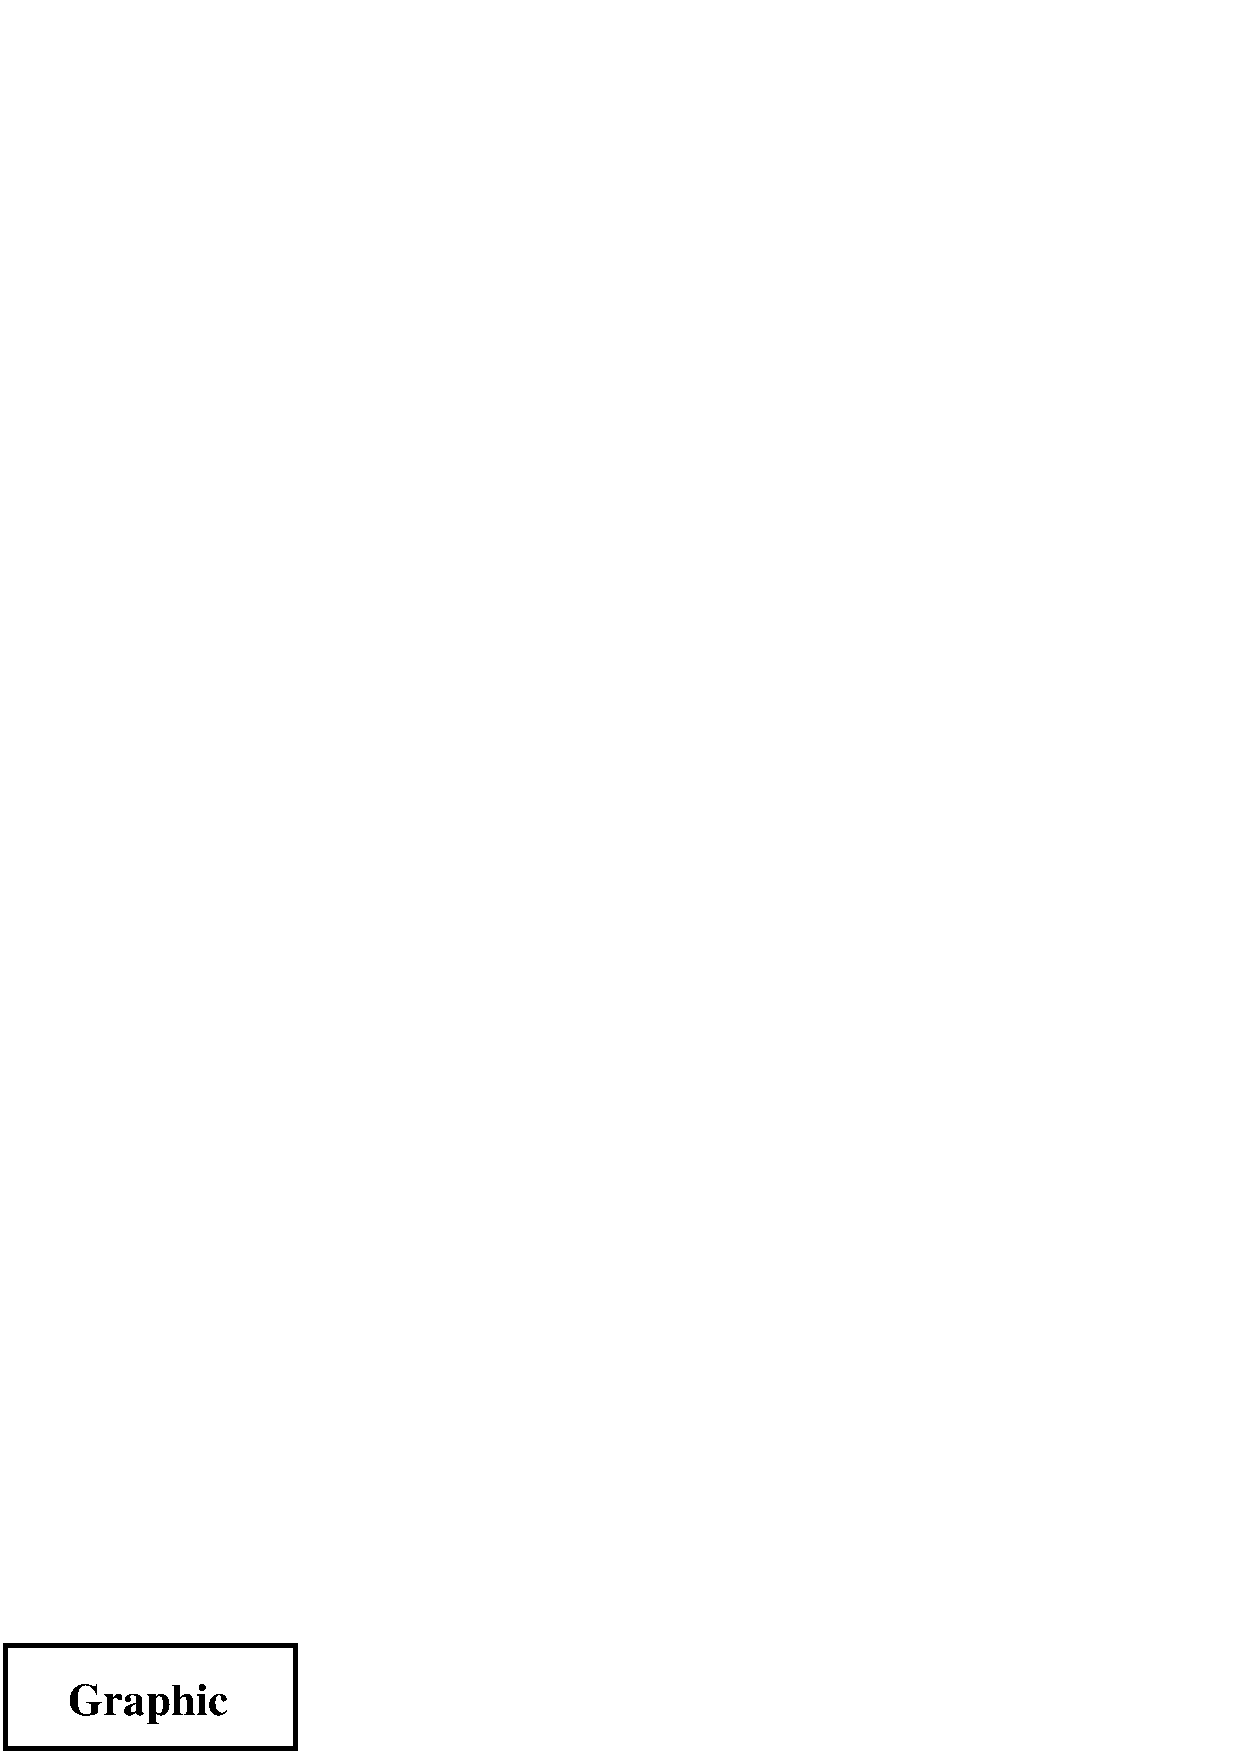
\includegraphics[angle=90,totalheight=1cm]{graphic}
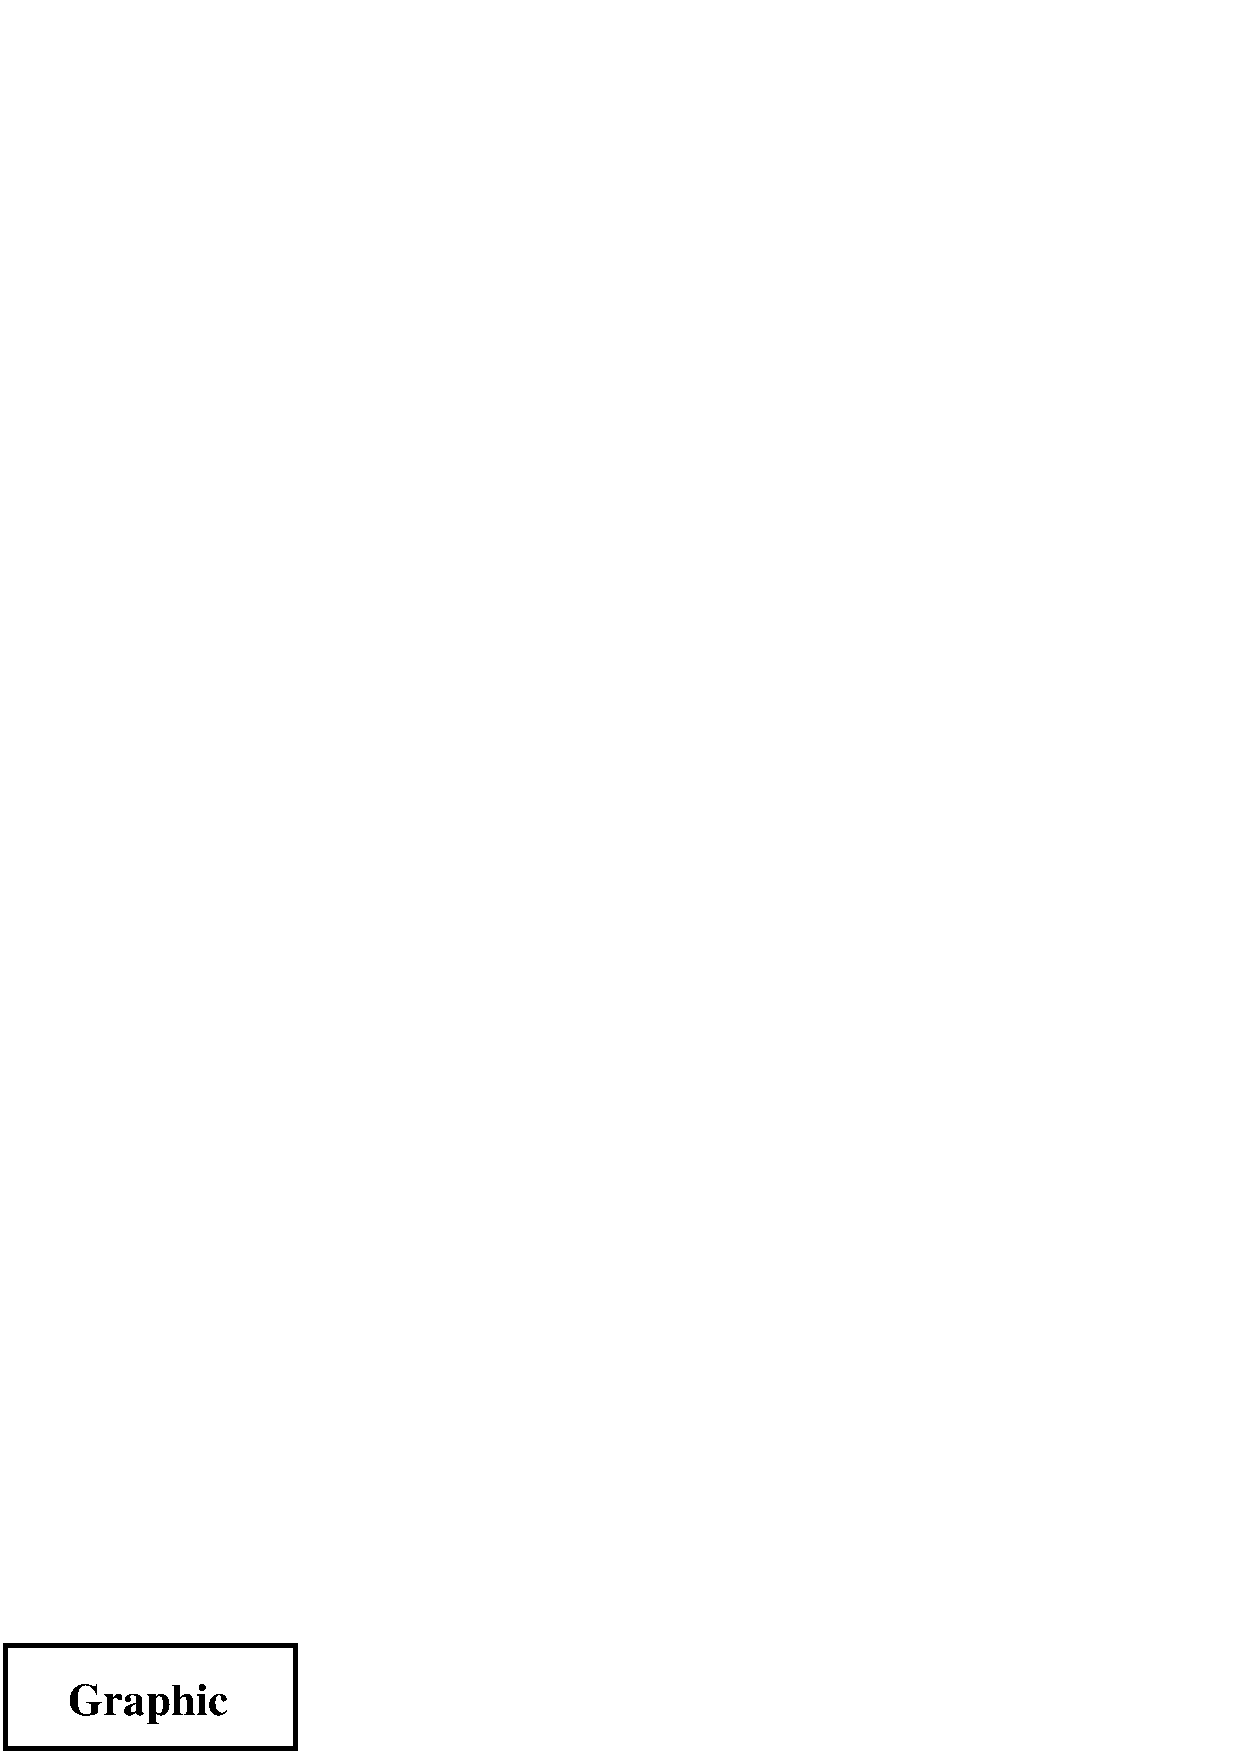
\includegraphics[totalheight=1cm,angle=90]{graphic}
\end{center}
\end{lstlisting}
会生成如下结果
\begin{center}
	\resizebox*{!}{1cm}{\rotatebox{90}{\usebox{\boxgraphic}}}
	\rotatebox{90}{\resizebox*{!}{1cm}{\usebox{\boxgraphic}}}
\end{center}
第一个盒子是先旋转了90度,然后缩放使得整体高度为1厘米。
第二个盒子先缩放使得整体高度为1厘米,然后再旋转90度。
另外要注意的是,以上图形中两幅图像之间有一个空格,
因为第一行 \cmd{includegraphics} 的末尾并没有以 \texttt{\%} 结束。

\begin{table}
\centering
\caption{\cmd{includegraphics} 选项}\label{tab:opt}
\begin{tabular}{>{\ttfamily}l P{0.7\textwidth}}
	\toprule
	height & 图形的高度(可为任何~\TeX{}~度量单位)。 \\ \hline
	totalheight & 图形的整体高度,可为任何~\TeX{}~度量单位。 \\ \hline
	width & 图形的宽度(可为任何~\TeX{}~度量单位)。 \\ \hline
	scale & 图形的缩放因子,设定 \opt{scale=2} 会使插入图形的大小为其自然大小的两倍。 \\ \hline
	angle & 设定旋转的角度,以度为单位,逆时针方向为正。 \\ \hline
	origin & \opt{origin} 指定图形绕那一点旋转,默认是围绕参考点旋转。
		\opt{origin} 点可以与第~\ref{ssec:rotatebox}节的 \cmd{rotatebox} 命令中的一样。
	比如 \opt{origin=c} 将使图形绕它的中心旋转。  \\ \hline
	bb & 设定 BoundingBox 的值。
	例如,\opt{bb=10 20 100 200} 设定BoundingBox 的左下角在 $(10,20)$,右上角在 $(100,200)$。\par
	因为 \cmd{includegraphics} 会自动从 \file{eps} 文件中读入BoundingBox值,
	所以一般不用\opt{bb} 这个选项。
	但它在 \file{eps} 文件中的 BoundingBox 丢失或不准确时还是很有用的。 \\ 
	\bottomrule
\end{tabular}
\end{table}

\begin{table}
\centering
\caption{\cmd{includegraphics} 裁剪选项}\label{tab:cropopt}
\begin{tabular}{>{\ttfamily}l P{0.7\textwidth}}
	\toprule
	viewpoint & 指定图像可以被看到的部分。
	如同 BoundingBox 一样,这个区域由四个数字决定,分别是左下角和右上角的坐标。
	这里的坐标是以 BoundingBox 左下角为起点的相对坐标。
	
	例如,如果图像的 BoundingBox 的值是 \texttt{50	50 410 302},
	那么 \texttt{viewpoint=50 50 122 122} 将显示以图像左下角为左下角的一英寸大小的正方形区域。
	而 \texttt{viewpoint=338 230 410 302} 则会显示以图形的右上角为右上角的一英寸大小的正方形区域。
	
	必须使用\opt{clip} 选项(见表~\ref{tab:boolopt})来阻止显示视图以外的图形部分。 \\ \hline
	trim & 显示部分图像的另一种方法。
	所给出的四个数字分别代表了从左、下、右、上被截去的值。
	正数代表从此方向截去的大小,而负数则代表从此方向加上的大小。
	
	例如,\opt{trim=1 2 3 4} 代表图像的左边截去1 \texttt{bp},
	下边截去2 \texttt{bp},右边截去3 \texttt{bp},上边截去4 \texttt{bp}。
	
	必须使用\opt{clip} 选项(见表~\ref{tab:boolopt})来阻止显示被截去的部分。 \\ \bottomrule
\end{tabular}
\end{table}

\begin{table}
\centering
\caption{\cmd{includegraphics} 布尔型选项}\label{tab:boolopt}
\begin{tabular}{>{\ttfamily}l P{0.7\textwidth} }
	\toprule
	clip & 指定 \opt{clip=false} 会显示整个的图形,即使有些部分在视图之外。(默认值)
	
	指定 \opt{clip=true} 时将不显示图形在视图之外的部分。 \\ \hline
	draft & 当使用\opt{draft} 或 \opt{draft=true} 选项将阻止图像的导入。
	此时在插图的位置只显示图像的BoundingBox和文件名,
	这会加快文档的显示和打印速度。
	使用 \opt{draft=false} 则会显示图像。
	
	如果使用 \opt{draft} 宏包选项 \cmdOM{usepackage}{draft}{graphicx},
	那么文档中的所有图像都以\opt{draft} 方式插入。  \\ \hline
	keepaspectratio & 在没有设定\opt{keepaspectratio} 选项时,
	如果同时给定图像的宽度和高度/整体高度,
	那么为了满足所设定的高和宽,图像的缩放可能会失真变形。
	
	在设定\opt{keepaspectratio} 选项后,给定图像的宽度和高度/整体高度时,
	图像会在保持原有的宽高比例下缩放,尽可能使得图像满足所设定的高和宽,
	但是图像的实际宽高不会超出设置的值。 \\ \bottomrule
\end{tabular}
\end{table}


\subsection{一些例子}

下面是一些使用 \cmd{includegraphics} 命令来插入图形的例子。
\footnote{
	本小节来自于王磊在旧版本的中译本《\LaTeXe{} 插图指南》中额外补充的内容。——译注}
这里为方便起见,定义水平线 \cmd{HR} 为
\begin{lstlisting}
\newcommand{\HR}{\rule{1em}{0.4pt}}
\end{lstlisting}

\ifxetex\relax\else\ifpdf\relax\else %因为使用pdflatex不支持clip.所以省去。
在下面的几个例子中可以看到使用\opt{bb,clip,viewport} 和\opt{trim}的效果。

\hspace{-1cm}\begin{minipage}[c]{.5\textwidth}
	左\HR%
	\fbox{%
		
\includegraphics[bb=120 120 150 200]{w.eps}}%
	\HR 右
	\qquad
	左\HR%
	\fbox{%
		
\includegraphics[bb=120 120 150 200,clip]{w.eps}}%
	\HR 右
\end{minipage}%
\begin{minipage}[c]{.5\textwidth}
	\begin{Verbatim}[frame=lines,label=\colorbox{green}{\small 例一},labelposition=topline,]
	左\HR\fbox{%
	\includegraphics
	[bb=120 120 150 200]%
	{w.eps}}%
	\HR 右
	\qquad
	左\HR\fbox{%
	\includegraphics
	[bb=120 120 150 200,clip]%
	{w.eps}}%
	\HR 右
	\end{Verbatim}
\end{minipage}

\hspace{-1.5cm}\begin{minipage}[c]{.65\textwidth}
	左\HR\fbox{%
		
\includegraphics[viewport=20 20 50 100,clip]{w}}%
	\HR 右
	\qquad
	左\HR\fbox{%
		
\includegraphics[trim=5 5 10 10,clip]{w}}%
	\HR 右
\end{minipage}%
\hspace{-1cm}\begin{minipage}[c]{.5\textwidth}
	\begin{Verbatim}[frame=lines,label=\colorbox{green}{\small 例二},labelposition=topline]
	左\HR\fbox{%
	\includegraphics
	[viewport=20 20 50 100,clip]%
	{w.eps}}%
	\HR 右
	\qquad
	左\HR\fbox{%
	\includegraphics
	[trim=5 5 10 10,clip]%
	{w.eps}}
	\HR 右
	\end{Verbatim}
	\par\vspace{0pt}
\end{minipage}
\fi\fi

在下面的几个例子中,可以比较以下使用 \opt{scale,width,height,angle} 以及 \opt{keepaspectratio} 选项及其不同的顺序所得到的不同效果。

\begin{minipage}[t]{.45\textwidth}
	\vspace{0pt}
	左\HR\fbox{%
		\scalebox{0.5}{\usebox{\boxw}}}\HR 右
\end{minipage}%
\hspace{-.5cm}
\begin{minipage}[t]{.5\textwidth}
	\vspace{0pt}
\begin{Verbatim}[frame=lines,label=\colorbox{green}{\small 例一},labelposition=topline]
左\HR\fbox{%

\includegraphics
[scale=.5]{w.eps}%
\HR 右
\end{Verbatim}
\end{minipage}

\begin{minipage}[c]{.45\textwidth}
	左\HR\fbox{%
		\resizebox{10mm}{!}{\usebox{\boxw}}}\HR 右
\end{minipage}%
\hspace{-.5cm}
\begin{minipage}[c]{.5\textwidth}
\begin{Verbatim}[frame=lines,label=\colorbox{green}{\small 例二},labelposition=topline]
左\HR\fbox{%
\includegraphics%
[width=10mm]{w.eps}%
\HR 右
\end{Verbatim}
\end{minipage}

\begin{minipage}[c]{.45\textwidth}
	左\HR\fbox{%
		\resizebox{20mm}{30mm}{\usebox{\boxw}}}\HR 右
\end{minipage}%
\hspace{-.5cm}
\begin{minipage}[c]{.5\textwidth}
\begin{Verbatim}[frame=lines,label=\colorbox{green}{\small 例三},labelposition=topline]
左\HR\fbox{%
\includegraphics
[height=20mm,width=30mm]%
{w.eps}}\HR 右
\end{Verbatim}
\end{minipage}

\begin{minipage}[c]{.45\textwidth}
	左\HR\fbox{%
		
\includegraphics[height=20mm,width=30mm,%
		keepaspectratio]{w}}\HR 右
\end{minipage}%
\hspace{-.5cm}
\begin{minipage}[c]{.5\textwidth}
\begin{Verbatim}[frame=lines,label=\colorbox{green}{\small 例四},labelposition=topline]
左\HR\fbox{%

\includegraphics
[height=20mm,width=30mm,%
keepaspectratio]{w.eps}}%
\HR 右
\end{Verbatim}
\end{minipage}

\begin{minipage}[c]{.45\textwidth}
	左\HR\fbox{%
		\rotatebox{-45}{\usebox{\boxw}}}\HR 右
\end{minipage}%
\hspace{-.5cm}
\begin{minipage}[c]{.5\textwidth}
\begin{Verbatim}[frame=lines,label=\colorbox{green}{\small 例五},labelposition=topline]
左\HR\fbox{%

\includegraphics
[angle=-45]{w.eps}}%
\HR 右
\end{Verbatim}
\end{minipage}

\begin{minipage}[c]{.45\textwidth}
	左\HR\fbox{%
		\resizebox{30mm}{!}{\rotatebox{-45}{\usebox{\boxw}}}}\HR 右
\end{minipage}%
\hspace{-.5cm}
\begin{minipage}[c]{.5\textwidth}
\begin{Verbatim}[frame=lines,label=\colorbox{green}{\small 例六},labelposition=topline]
左\HR\fbox{%
\includegraphics
[angle=-45,width=30mm]%
{w.eps}}\HR 右
\end{Verbatim}
\end{minipage}

\hspace{-1cm}
\begin{minipage}[c]{.45\textwidth}
	左\HR\fbox{%
		\rotatebox{-45}{\resizebox{30mm}{!}{\usebox{\boxw}}}}\HR 右
\end{minipage}%
\begin{minipage}[c]{.5\textwidth}
\begin{Verbatim}[frame=lines,label=\colorbox{green}{\small 例七},labelposition=topline]
左\HR\fbox{%
\includegraphics
[width=30mm,angle=-45]%
{w.eps}}\HR 右
\end{Verbatim}
\end{minipage}

\begin{minipage}[c]{.45\textwidth}
	左\HR\fbox{%
		\resizebox*{!}{15mm}{\rotatebox{-60}{\usebox{\boxw}}}}%
	\HR 右
\end{minipage}%
\hspace{-.5cm}
\begin{minipage}[c]{.5\textwidth}
\begin{Verbatim}[frame=lines,label=\colorbox{green}{\small 例八},labelposition=topline]
左\HR\fbox{%
\includegraphics
[angle=-60,totalheight=15mm]%
{w.eps}}%
\HR 右
\end{Verbatim}
\end{minipage}

\begin{minipage}[c]{.45\textwidth}
	左\HR\fbox{%
		\resizebox*{30mm}{20mm}{\rotatebox{-60}{\usebox{\boxw}}}}%
	\HR 右
\end{minipage}%
\hspace{-.5cm}
\begin{minipage}[c]{.5\textwidth}
\begin{Verbatim}[frame=lines,label=\colorbox{green}{\small 例九},labelposition=topline]
左\HR\fbox{%

\includegraphics
[angle=-60,totalheight=20mm,%
width=30mm]{w.eps}}%
\HR 右
\end{Verbatim}
\end{minipage}

\begin{minipage}[c]{.45\textwidth}
	左\HR\fbox{%
		
\includegraphics[angle=-60,totalheight=20mm,width=30mm,keepaspectratio]{w}}%
	\HR 右
\end{minipage}%
\hspace{-.5cm}
\begin{minipage}[c]{.5\textwidth}
\begin{Verbatim}[frame=lines,label=\colorbox{green}{\small 例十},labelposition=topline]
	左\HR\fbox{%
	\includegraphics
	[angle=-60,totalheight=20mm,%
	width=30mm,keepaspectratio]%
	{w.eps}}%
	\HR 右
\end{Verbatim}
\end{minipage}

\section{旋转和缩放对象}\label{sec:scalerotate}
除了 \cmd{includegraphics}命令外,
\pkg{graphicx} 宏包还提供了另外四个命令用来旋转和缩放任意的 \LaTeX{} 对象,例如文本、图像等。
\begin{lstlisting}
\scalebox{水平缩放因子}[垂直缩放因子]{对象}
\resizebox{宽度}{高度}{对象}
\resizebox*{宽度}{整体高度}{对象}
\rotatebox[选项]{角度}{对象}
\end{lstlisting}

因为 \pkg{graphicx} 包的 \cmd{includegraphics} 已经带有 \opt{angle}、\opt{width} 等支持旋转和缩放的选项,
所以本节介绍的这几个命令很少在插图时使用。例如:
\begin{lstlisting}
\includegraphics[scale=2]{file.eps}
\includegraphics[width=4in]{file.eps}
\includegraphics[angle=45]{file.eps}
\end{lstlisting}
上述命令和下面的命令等到的结果是相同的。
\begin{lstlisting}
\scalebox{2}{\includegraphics{file.eps}}
\resizebox{4in}{!}{\includegraphics{file.eps}}
\rotatebox{45}{\includegraphics{file.eps}}
\end{lstlisting}

尽管结果相同,但在最好还是用前一种方法,
因为它的速度更快,而且生成的 PostScript 和 \file{pdf} 效率更高。

\subsection{scalebox 命令}\label{ssec:scalebox}
语法:
\begin{lstlisting}
\scalebox{水平缩放因子}[垂直缩放因子]{对象}
\end{lstlisting}

\cmdi{scalebox} 命令对其作用的对象进行缩放,
使得缩放后对象的宽度为原始宽度与\texttt{水平缩放因子}之积,高度为原始高度与\texttt{垂直缩放因子}之积。
如果\texttt{垂直缩放因子}没有给出,那么默认取为\texttt{水平缩放因子},
以保持原始的宽高比进行缩放。
如果缩放因子为负值,则对对象进行翻转。下面是几个例子

\hspace{-1.5cm}
\begin{minipage}[b]{.5\textwidth}
	\begin{center}
		\color{blue}{\CJKfamily{zhkai}
			\scalebox{2}{这是放大的文字} \\
			这是正常的文字 \\
			\scalebox{.5}{这是缩小的文字}}
	\end{center}
	\par\vspace{0pt}
\end{minipage}%
\begin{minipage}[b]{.5\textwidth}
\begin{lstlisting}
\scalebox{2}{这是放大的文字} \\
这是正常的文字  \\
\scalebox{.5}{这是缩小的文字}
\end{lstlisting}
\par\vspace{0pt}
\end{minipage}

\hspace{-1.5cm}
\begin{minipage}[b]{.5\textwidth}
	\color{blue}{\CJKfamily{zhkai}
		\framebox{\scalebox{2}{%
				\parbox{.5in}{放大 \\ 和 \\ 缩小}}}
		\framebox{\scalebox{2}[1.5]{%
				\parbox{.5in}{放大 \\ 和 \\ 缩小}}}}
	\par\vspace{0pt}
\end{minipage}%
\begin{minipage}[b]{.5\textwidth}
\begin{lstlisting}
\framebox{\scalebox{2}{%
\parbox{.5in}{放大 \\ 和 \\ 缩小}}}
\framebox{\scalebox{2}[1.5]{%
\parbox{.5in}{放大 \\ 和 \\ 缩小}}}
\end{lstlisting}
\par\vspace{0pt}
\end{minipage}

\hspace{-1.5cm}
\begin{minipage}[b]{.5\textwidth}
	\begin{center}
		\color{blue}{\texttt{%
				China? \scalebox{-1}[1]{China?} \\
				China? \scalebox{1}[-1]{China?} \\
				China? \scalebox{-1}[-1]{China?} \\
				China? \scalebox{-1}{China?}}}
	\end{center}
	\par\vspace{0pt}
\end{minipage}%
\begin{minipage}[b]{.5\textwidth}
\begin{lstlisting}
China? \scalebox{-1}[1]{China?} \\
China? \scalebox{1}[-1]{China?} \\
China? \scalebox{-1}[-1]{China?} \\
China? \scalebox{-1}{China?}}
\end{lstlisting}
\par\vspace{0pt}
\end{minipage}

\subsection{resizebox 命令}\label{ssec:resizebox}
语法:
\begin{lstlisting}
\resizebox{宽度}{高度}{对象}
\resizebox*{宽度}{整体高度}{对象}
\end{lstlisting}

\cmdi{resizebox} 命令将对象的大小改变为给定值。
如果\texttt{宽度}或\texttt{高度}中的任一项用 \texttt{!} 给出,
那么缩放时会保持原有的宽高比。
例如:
\begin{lstlisting}
\resizebox{2in}{!}{argument}
\end{lstlisting}
将对象的宽度改变为2英寸,同时保持宽高比。

标准的 \LaTeXe{} 长度命令 \cmd{height}、\cmd{width}、\cmd{totalheight}、\cmd{depth} 可用来表示对象的原始尺寸。
因此,
\begin{lstlisting}
\resizebox{2in}{\height}{argument}
\end{lstlisting}
使得对象的宽度改变为 2 英寸但保持原有高度不变。 

除了以外,
命令 \cmdi{reseizebox*} 与 \cmd{resizebox} 几乎是相同的
不同之处仅在于第二个参数表示对象的全部高度
(关于高度和整体高度的定义见第~\ref{sec:terminology} 节,
关于 \opt{height} 和 \opt{totalheight} 选项的比较见第~\ref{ssec:diffheight} 节。)

下面是几个例子:

\hspace{-1.5cm}\begin{minipage}[b]{.5\textwidth}
	\begin{center}
		\color{blue}{\CJKfamily{zhkai}
			\framebox{\resizebox{5mm}{!}{%
					\parbox{14mm}{选项 \\ 角度 \\ 对象}}}
			\framebox{\resizebox{!}{10mm}{%
					\parbox{14mm}{选项 \\ 角度 \\ 对象}}}}
		\par\vspace{0pt}
	\end{center}
\end{minipage}%
\hspace{-1cm}\begin{minipage}[b]{.5\textwidth}
\begin{lstlisting}
\framebox{\resizebox{5mm}{!}{%
\parbox{14mm}{选项 \\ 角度 \\ 对象}}}
\framebox{\resizebox{!}{10mm}{%
\parbox{14mm}{选项 \\ 角度 \\ 对象}}}
\end{lstlisting}
\par\vspace{0pt}
\end{minipage}

\hspace{-2cm}
\begin{minipage}[b]{.5\textwidth}
	\begin{center}
		\color{blue}{\CJKfamily{zhkai}
			\resizebox*{2cm}{3cm}{\LaTeX{}~图形} \\
			\resizebox*{2cm}{1cm}{\LaTeX{}~图形}}
		\par\vspace{0pt}
	\end{center}
\end{minipage}%
\begin{minipage}[b]{.5\textwidth}
\begin{lstlisting}
\resizebox*{2cm}{3cm}{\LaTeX{}~图形} \\
\resizebox*{2cm}{1cm}{\LaTeX{}~图形}
\end{lstlisting}
\par\vspace{0pt}
\end{minipage}

\subsection{rotatebox 命令}\label{ssec:rotatebox}
语法:
\begin{lstlisting}
\rotatebox[选项]{角度}{对象}
\end{lstlisting}
\cmdi{rotatebox} 将对象旋转一给定度数的角度,逆时针方向为正。
默认\texttt{选项}下对象绕它的参考点旋转。
\cmd{rotatebox} 命令中\texttt{选项} 允许对象绕给定的点来旋转。
\begin{enumerate}
	\item 给定\opt{[x=xdim,y=ydim]},则对象旋转所绕的点相对于参考点的
	坐标为 $(\mathtt{xdim}, \mathtt{ydim})$。
	\item \opt{origin} 选项可以指定12个特殊点其中之一(见图~\ref{fig:rotatepoint})。
\end{enumerate}

\opt{origin} 点的水平位置由\opt{lcr} (分别代表左、中、右)三个字母其中之一确定,
垂直位置则由\opt{t,c,B,b}~(分别代表顶部、中部、基线、底部)四个字母中的一个来确定。
例如:
\begin{description}
	\item [\opt{[rb]}] 右下角。
	\item [\opt{[lt]}] 左上角。
	\item [\opt{[cB]}] 图形基线的中点。
\end{description}

\paragraph{几点说明:}
\begin{itemize}
	\item 标记字母的顺序并不重要,\opt{[br]} 等同于 \opt{[rb]}。
	\item \opt{c}~代表水平位置的中点还是垂直位置的中点由和它一起的标记字母来决定。
	\item 如果只给出一个标记字母,那么另一个将被假设为 \opt{c}。
	即,\opt{[c]} 等于\opt{[cc]},\opt{[l]}等于\opt{[lc]},\opt{[t]}等于\opt{[ct]},等等。
\end{itemize}

\begin{figure}
	\centering
	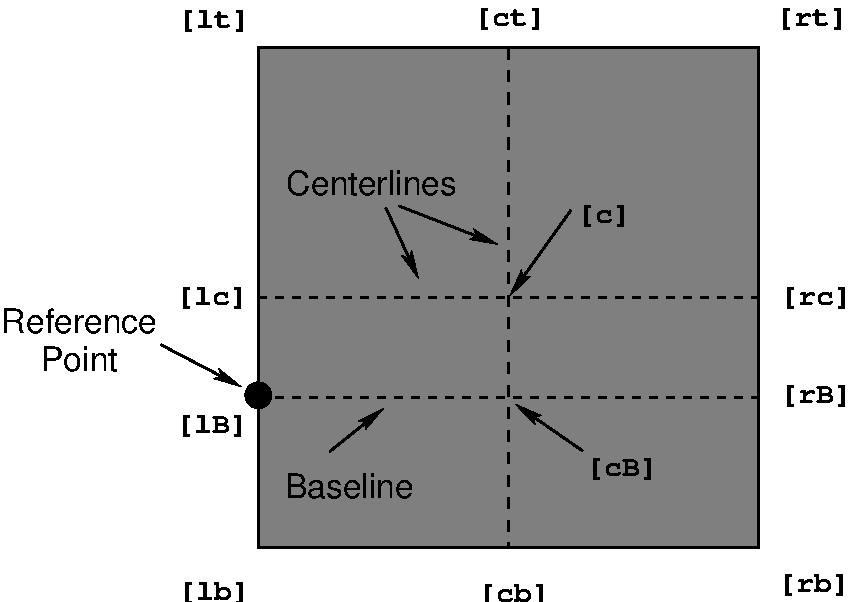
\includegraphics[width=.6\textwidth]{orig-point}
	\caption{可用的 \opt{origin} 点}\label{fig:rotatepoint}
\end{figure}

下面是一个例子:

\hspace{-1.5cm}
\begin{minipage}[b]{.5\textwidth}
	\begin{center}
		\setlength{\fboxsep}{0mm}
		\newcommand{\MyRot}[1]{%
			\fbox{\rotatebox{#1}{旋转~$#1^\circ$}}}
		\color{blue}{\CJKfamily{zhkai}
			\MyRot{0} \MyRot{45} \MyRot{90}
			\MyRot{135} \MyRot{180} \MyRot{225}}
	\end{center}
	\par\vspace{0pt}
\end{minipage}%
\begin{minipage}[b]{.5\textwidth}
\begin{lstlisting}
\setlength{\fboxsep}{0mm}
\newcommand{\MyRot}[1]{%
\fbox{\rotatebox{#1}{旋转~$#1^\circ$}}}
\MyRot{0} \MyRot{45} \MyRot{90}
\MyRot{135} \MyRot{180} \MyRot{225}
\end{lstlisting}
\par\vspace{0pt}
\end{minipage}


\section{高级插图命令}\label{sec:adgraphcmd}
本节描述了一些 \LaTeXe{} 图形宏包套件的高级命令,
用于下述情形。
\begin{enumerate}
	\item 当使用没有扩展名的文件名时。如:
\begin{lstlisting}
\includegraphics{file}
\end{lstlisting}

	\item 当使用压缩的\file{eps} 图形文件时。见第~\ref{ssec:compresseps}~节。
	\item 当使用非\file{eps} 格式的图形文件时。见第~\ref{ssec:noneps}~节。
\end{enumerate}
在这些情况下,\LaTeX{} 为了处理由 \cmd{includegraphics} 所引入的文件,
就需要用 \cmdi{DeclareGraphicsRule} 和 \cmdi{DeclareGraphicsExtensions} 命令来控制。
\begin{itemize}
	\item \cmd{DeclareGraphicsExtensions} 命令指定了在没有提供图形文件扩展名的情况下,
	\LaTeX{} 将自动为其加上的扩展名列表(如~\file{.eps}、\file{.ps}、\file{.eps.gz} 等)。
	\item \cmd{DeclareGraphicsRule} 命令指定了对图形文件执行的命令。
	执行这一命令要求操作系统支持管道功能,比如 Unix 等操作系统,而DOS则不行。
	
	若将此命令指定为一解压缩命令,那么就可以使用压缩的 \file{eps} 图形文件。
	若将此命令指定为一图形格式转换命令,那么就可以使用非\file{eps} 格式的图形文件。
\end{itemize}

\subsection{DeclareGraphicsExtensions 命令}\label{ssec:deextension}
\cmd{DeclareGraphicsExtensions} 命令告诉 \LaTeX{},
若~\cmd{includegraphics}~命令所引入的文件没有提供扩展名,
将试图为其自动加上什么样的扩展名。

为方便起见,在选择图形驱动
\footnote{
	指定一个图形驱动选项如 \cmdOM{usepackage}{dvips}{graphics} 将会覆盖掉在~\texttt{graphics.cfg} 中设定的缺省驱动选项——旧译本注。}
时,就已经有一个相应的预设扩展名集。
举例来说,如果选择 \prgname{dvips} 作为图形驱动,
那么默认会使用下列图形文件扩展名(在~\file{dvips.def}~中定义):
\begin{lstlisting}
\DeclareGraphicsExtensions{.eps,.ps,.eps.gz,.ps.gz,.eps.Z}
\end{lstlisting}

如果 \pkg{graphicx} 宏包使用 \prgname{pdftex} 驱动,
那么默认会使用下列图形文件扩展名(在 \file{pdftex.def} 中定义)
\cprotect\footnote{
	实际上在最新版本(2016年)中,\file{dvips.def} 中定义扩展名的方式为
\begin{lstlisting}
%\def\Gin@extensions{.eps,.ps,.eps.gz,.ps.gz,.eps.Z,.mps}
\end{lstlisting}
	\file{pdftex.def} 中定义扩展名的方式为
\begin{lstlisting}
\def\Gin@extensions{.png,.pdf,.jpg,.mps,.jpeg,.PNG,.PDF,.JPG,.JPEG}
\end{lstlisting}
	——译注}:
\begin{lstlisting}
\DeclareGraphicsExtensions{.png,.pdf,.jpg,.mps}
\end{lstlisting}

在 \opt{dvips} 图像扩展名列表中,
\cmdM{includegraphics}{file} 首先寻找 \file{file.eps},
其次是 \file{file.ps},再其次是 \texttt{file.eps.gz},直到找到一个文件。
相应地,可以用
\begin{lstlisting}
\includegrapincs{file}
\end{lstlisting}
取代
\begin{lstlisting}
\includegrapincs{file.eps}
\end{lstlisting}
这样做的好处是如果以后决定压缩 \file{file.eps},也无须更改 \LaTeX{} 文件。
无后缀名的方式使得可以同时使用 \LaTeX{} 和 \pdfLaTeX{} 编译文档,
见第~\pageref{ssec:latexandpdflatex} 页的~\ref{ssec:latexandpdflatex} 节。
然而,这种无后缀名的方式可能会加剧内存池空间问题,详见下面的~\ref{sssec:poolspaceproblem} 小节。

\subsubsection{无扩展名的文件}
需要注意的是,
\begin{lstlisting}
\includegrapincs{file}
\end{lstlisting}
不会试图寻找~\file{file},
除非空扩展名列表中包含空的扩展名 \verb+{}+。
例如:
\begin{lstlisting}
\DeclareGraphicsExtensions{.eps,.eps.gz,{}}
\end{lstlisting}
将试图在没找到 \file{file.eps} 和 \file{file.eps.gz} 的情况下寻找 \file{file}。

由于默认的扩展名列表中不包含空扩展名,
如果想要使用无扩展名文件的话,
必须使用 \cmd{DeclareGraphicsExtensions} 命令定义一个包含空扩展名的列表。

\subsubsection{池空间问题}\label{sssec:poolspaceproblem}

不给出扩展名而靠 \LaTeX{} 从 \cmd{DeclareGraphicsExtensions} 的扩展名列表中选择正确的扩展名可能
加剧池空间问题(见第~\ref{ssec:poolspace}~节)。
如果有池空间问题的话,应当使用 \cmd{DeclareGraphicsExtensions} 指定的扩展名数目尽可能小。如:
\begin{lstlisting}
\DeclareGraphicsExtensions{.eps,.eps.gz}
\end{lstlisting}


\subsection{DeclareGraphicsRule 命令}\label{ssec:derule}
\cmdi{DeclareGraphicsRule} 命令指定 \cmd{includegraphics} 如何按照扩展名
来对操作图像文件。语法为
\begin{lstlisting}
\DeclareGraphicsRule{ext}{type}{sizefile}{command}
\end{lstlisting}
例如,如下命令
\begin{lstlisting}
\DeclareGraphicsRule{.eps.gz}{eps}{.eps.bb}{`gunzip -c #1}
\end{lstlisting}
指定任何以 \file{.eps.gz} 为扩展名的文件为压缩的\file{eps} 文件,
该文件的 BoundingBox 信息存放在扩展名为 \file{.eps.bb} 的文件中,
并用命令 \texttt{gunzip -c} 来解压缩
(因为 \LaTeX{} 不能从压缩文件中读取 BoundingBox~信息,
所以 BoundingBox 行必须存放到非压缩文件中)。

可以允许有多个 \cmd{DeclareGraphicsRule} 命令。

\cmd{DeclareGraphicsRule} 命令允许使用 \texttt{*} 代表任何未知扩展名,
例如:
\begin{lstlisting}
\DeclareGraphicsRule{*}{eps}{*}{}
\end{lstlisting}
会导致所有未知扩展名的文件都被认为是 \file{eps} 文件,
比方说 \file{file.EPS} 就被当做\file{eps} 文件。

\begin{table}
	\centering
	\caption{\cmd{DeclareGraphicsRule} 的选项}\label{tab:DeclaregruleArgs}
	\kaishu 
	\begin{tabular}{>{\ttfamily}l  P{0.7\textwidth}}
		\toprule
		ext & 文件的扩展名。 \\ \hline
		type & 扩展名所对应的图像类型。 \\ \hline
		sizefile & 包含图像 BoundingBox 信息的文件的扩展名。
		如果这一选项为空,
		那么必须要在 \cmd{includegraphics} 命令中给定 \opt{bb} 选项的值。 \\ \hline
		command & 作用于图像文件的命令,此项常为空。
		命令前必须有一个前单引号(键盘上数字键 \texttt{1} 的左侧键——译注),
		注意不是常用的后单引号。
		目前为止,只有 \prgname{dvips} 能够执行这样的命令。
		参见第~\ref{ssec:noneps}~节关于如何用这样的命令来处理非 \file{eps} 格式图像和压缩的 \file{eps} 图像的例子。\\
		\bottomrule
	\end{tabular}
\end{table}

文件的扩展名定义为文件名里第一个句点以后的部分,
\marginpar{文件名中的句点}
这样做是为了可以将 \file{.eps.gz} 结尾的文件识别成压缩的\file{eps} 文件。
为了避免混淆,文件的基本名中不要使用句点。
例如,指定文件 \file{file.name.eps.gz} 会让 \cmd{includegraphics} 寻找扩展名为 \file{.name.eps.gz} 所对应的图像规则。
由于这样的规则很有可能不存在,结果导致使用未知扩展名所对应的规则。
例外的情形是该文件的格式正好是缺省格式,
如果未知扩展名的文件都被认为是 \file{eps} 文件,
那么 \file{file.name.eps} 就恰巧能被正确地识别。

为方便起见,根据不同的图形驱动选项,
\marginpar{预定义命令}
已经预定义了不同的缺省图像规则。
例如使用 \opt{dvips} 图形驱动选项时,文件 \file{dvips.def} 定义了如下缺省图形规则
\footnote{
	实际上 \file{dvips.def} 的代码并没有使用 \cmd{DeclareGraphicsRule},
	不过效果是一样。}:
\begin{lstlisting}
\DeclareGraphicsRule{.eps}{eps}{.eps}{}
\DeclareGraphicsRule{.ps}{eps}{.ps}{}
\DeclareGraphicsRule{.pz}{eps}{.bb}{`gunzip -c #1}
\DeclareGraphicsRule{.eps.Z}{eps}{.eps.bb}{`gunzip -c #1}
\DeclareGraphicsRule{.ps.Z}{eps}{.ps.bb}{`gunzip -c #1}
\DeclareGraphicsRule{.eps.gz}{eps}{.eps.bb}{`gunzip -c #1}
\DeclareGraphicsRule{.ps.gz}{eps}{.ps.bb}{`gunzip -c #1}
\DeclareGraphicsRule{.pcx}{bmp}{}{}
\DeclareGraphicsRule{.bmp}{bmp}{}{}
\DeclareGraphicsRule{.msp}{bmp}{}{}
\DeclareGraphicsRule{*}{eps}{*}{}
\end{lstlisting}
前面两个命令定义扩展名为 \file{.eps} 和 \file{.ps} 的文件为 \file{eps} 文件,
它们后面的五个命令定义了压缩 \file{eps} 文件的扩展名和解压命令,
接下来的三个命令定义了位图文件 \file{pcx}、\file{bmp}、\file{msp} 的扩展名,
最后一个命令设定未知扩展名的文件按照 \file{eps} 文件处理。

如果使用 \pdfTeX 引擎,那么 \file{pdftex.def} 缺省定义了以下的图形规则
\footnote{
	\file{pdftex.def} 实际上先检查 \pdfTeX{} 的版本,
	然后根据不同版本的处理方式定义相应的图形规则。}:
\begin{lstlisting}
\DeclareGraphicsRule{.png}{png}{.png}{}
\DeclareGraphicsRule{.pdf}{pdf}{.pdf}{}
\DeclareGraphicsRule{.jpg}{jpg}{.jpg}{}
\DeclareGraphicsRule{.mps}{mps}{.mps}{}
\end{lstlisting}
这样就指定了 \pdfTeX{} 支持的图像格式的处理方式。

\clearpage
\endinput

